\documentclass[10pt,a4paper,headinclude,twoside, plainheadsepline, open=right, numbers=noenddot, twocolumn]{article}

%
%\addto\captionsgerman{\renewcommand{\figurename}{Fig.}}
%
%%%%%%%%%%%%%%%%%%%%%%%%%%%%%%%%%%%%%%%%%%%%%%%%%%%%%%%%%%%
%
% Literaturverzeichnis
%
% Hier eine von zwei Varianten auswaehlen:
% Nummern oder Buchstaben fuer Referenzen
%\usepackage[backend=biber, style=alphabetic, sorting=nyt]{biblatex}
\usepackage[backend=biber, style=numeric-comp, sorting=none]{biblatex}
%
% Hier werden die Referenzen in einer separaten Datei gespeichert
\addbibresource{termPaper.bib}
%
% WICHTIG: Hier wird nicht BibTeX sondern BibLateX verwendet!!
% Deshalb nicht mit bibtex uebersetzen, sondern mit biber
% Das kann man in jedem Tool wie TexMaker oder TexShop als Option einstellen
%

% Spezielle Einstellungen, insbesondere fuer das Literaturverzeichnis,
% aber auch Packages wie amsmath, Groessenanpassungen etc.
% Allgemeines
%\usepackage[automark]{scrpage2} % Kopf- und Fusszeilen
\usepackage{amsmath} % Mathematik
\usepackage{amsfonts}
\usepackage{amssymb}
\usepackage[utf8]{inputenc} % UTF8-Kodierung fuer Umlaute usw
\usepackage{hyperref} % Internetseiten
\usepackage{multirow} % Tabellen-Zellen ueber mehrere Zeilen
\usepackage{multicol} % mehre Spalten auf eine Seite
\usepackage{tabularx} % Fuer Tabellen mit vorgegeben Groessen
\usepackage[ngerman]{babel}
\usepackage{graphicx} % Bilder
\usepackage{epstopdf} % enable eps graphics
\usepackage{color} % Farben
\usepackage{subfig} % mehrere Abbildungen nebeneinander/uebereinander
% Quellcode
\usepackage{listings} % fuer Formatierung in Quelltexten
\usepackage[font=small,labelfont=bf,figurename=Abb.,tablename=Tab.]{caption}
\usepackage{capt-of}
%%%%%%%%%%%%%%%%%%%%%%%%%%%%%%%%%%%%%%%%%%%%%%%%%%%%%%%%%%%
% ------
% Fonts and typesetting settings
\usepackage[sc]{mathpazo}
\usepackage[T1]{fontenc}
\usepackage{microtype}
% ------
% Page layout
\usepackage[hmarginratio=1:1,top=32mm,columnsep=20pt]{geometry}
\usepackage[font=it]{caption}
\usepackage{paralist}

% ------
% Abstract
\usepackage{abstract}
	\renewcommand{\abstractnamefont}{\normalfont\bfseries}
	\renewcommand{\abstracttextfont}{\normalfont\small\itshape}
%
%
% ------
% Titling (section/subsection)
\usepackage{titlesec}
\titleformat{\section}[block]{\large\scshape\centering}{\thesection.}{1em}{}
%
%%%%%%%%%%%%%%%%%%%%%%%%%%%%%%%%%%%%%%%%%%%%%%%%%%%%%%%%%%%
%
% Einstellungen zum Literaturverzeichnis
%
% Anpassen bei "alphabetic"
\ExecuteBibliographyOptions{%
     maxbibnames=99,   % Alle Autoren (kein et al.)
     maxcitenames=1,   % Kuerzel nur aus 1. Autor im Text
     maxalphanames=1,  % nur 1. Autor in der Abkuerzung
     backref=false,    % keine Ruueckverweise auf Zitatseiten
     firstinits=true,  % Vornamen abkuerzen
     isbn=false,       % ISBN ausblenden
     doi=false,        % DOI ausblenden
   }
\renewcommand*{\labelalphaothers}{} % alpha label ohne +
%
\renewbibmacro*{volume+number+eid}{%
     \setunit{\space}\printfield{volume}%
     \iffieldundef{number}{}{%
      \printtext[parens]{\printfield{number}}}%
     \setunit{\addcomma\space}\printfield{eid}}
%
% no word 'pages' for articles in the bibliography (print as is)
\DeclareFieldFormat[article, inproceedings, incollection, unpublished]{pages}{#1} 
% no quotes for article titles (print as is)
\DeclareFieldFormat[article, inproceedings, incollection, online, unpublished]{title}{#1} 
%
\renewbibmacro*{date}{\printdate}
\renewbibmacro*{issue+date}{\usebibmacro{issue}}
\renewbibmacro*{publisher+location+date}{\printlist{publisher}}
%
   \setcounter{biburlnumpenalty}{9000}
   \setcounter{biburlucpenalty}{9000}
   \setcounter{biburllcpenalty}{9999}
%
% "In:" removed for articles; issue/date macros added after note+pages macro
\DeclareBibliographyDriver{article}{%
  \usebibmacro{bibindex}%
  \usebibmacro{begentry}%
  \usebibmacro{author/translator+others}%
  \setunit{\labelnamepunct}\newblock%
  \usebibmacro{title}%
  \newunit%
  \printlist{language}%
  \newunit\newblock%
  \usebibmacro{byauthor}%
  \newunit\newblock%
  \usebibmacro{bytranslator+others}%
  \newunit\newblock%
  \printfield{version}%
  \newunit\newblock%
  \usebibmacro{journal+issuetitle}%
  \newunit%
  \usebibmacro{byeditor+others}%
  \newunit%
  \usebibmacro{note+pages}%
  \setunit{\addcomma\addspace}%
  \usebibmacro{date}%
  \usebibmacro{finentry}}
%
%
\DeclareBibliographyDriver{inproceedings}{%
    \usebibmacro{begentry}%
    \printnames{author}%
    \setunit{\labelnamepunct}\newblock%
    \printfield{title}%
    \setunit{\labelnamepunct}%
	\usebibmacro{in:}%    
    \newblock%
    \ifnameundef{editor}%
    {%
    		\setunit{\adddot\space}%
    		\newunit%
    }%
    {%
     	\setunit{\addspace}%
     	\printnames[byeditor]{editor}%
     	\clearname{editor}%
     	\setunit{\space}%
     	\printtext[parens]{Hrsg.}%
     	\setunit{\addcolon\space}%
     	\newunit%
     }%
	\printfield{booktitle}%
	\setunit{\addcomma\space}%
	\printfield{pages}%
	\setunit{\addcomma\space}%
    \usebibmacro{date}%
    \usebibmacro{finentry}
}

\DeclareBibliographyDriver{book}{%
  \usebibmacro{bibindex}%
  \usebibmacro{begentry}%
  \usebibmacro{author/editor+others/translator+others}%
  \setunit{\labelnamepunct}\newblock
  \usebibmacro{maintitle+title}%
  \newunit
  \printlist{language}%
  \newunit\newblock
  \usebibmacro{byauthor}%
  \newunit\newblock
  \usebibmacro{byeditor+others}%
  \newunit\newblock
  \printfield{edition}%
  \newunit
  \iffieldundef{maintitle}
    {\printfield{volume}%
     \printfield{part}}
    {}%
  \newunit
  \printfield{volumes}%
  \newunit\newblock
  \usebibmacro{series+number}%
  \newunit\newblock
  \printfield{note}%
  \newunit\newblock
  \usebibmacro{publisher+location+date}%
  \newunit\newblock
  \usebibmacro{chapter+pages}%
  \newunit
  \printfield{pagetotal}%
  \newunit\newblock
  \usebibmacro{doi+eprint+url}%
  \newunit\newblock
  \usebibmacro{addendum+pubstate}%
  \setunit{\bibpagerefpunct}\newblock
  \usebibmacro{pageref}%
  \setunit{\addcomma\space}
  \usebibmacro{date}
  \usebibmacro{finentry}}
%  
%
 \DeclareBibliographyDriver{online}{%
   \usebibmacro{bibindex}%
   \usebibmacro{begentry}%
   \ifnameundef{author}
    {\printtext{Autor unbekannt}}
    {
		\usebibmacro{author/editor+others/translator+others}%    
    }%
   \setunit{\labelnamepunct}\newblock
   \usebibmacro{title}%
   \newunitpunct
   \usebibmacro{url+urldate}%
   %\usebibmacro{addendum+pubstate}%
   \usebibmacro{finentry}}  
%%%%%%%%%%%%%%%%%%%%%%%%%%%%%%%%%%%%%%%%%%%%%%%%%%%%%%%%%%%

% Eigene Befehle %%%%%%%%%%%%%%%%%%%%%%%%%%%%%%%%%%%%%%%%%%%%%%%%%
% Matrix
\newcommand{\mat}[1]{
      {\textbf{#1}}
}
\newcommand{\todo}[1]{
      {\colorbox{red}{ TODO: #1 }}
}
\newcommand{\todotext}[1]{
      {\color{red} TODO: #1} \normalfont
}
\newcommand{\info}[1]{
      {\colorbox{blue}{ (INFO: #1)}}
}
\newcommand{\code}[1]{
      {\ttfamily{#1}}
}

%%%%%%%%%%%%%%%%%%%%%%%%%%%%%%%%%%%%%%%%%%%%%%%%%%%%%%
% Groessenanpassungen
%
\setlength{\unitlength}{1cm}
\setlength{\oddsidemargin}{0.3cm}
\setlength{\evensidemargin}{0.3cm}
\setlength{\textwidth}{15.5cm}
\setlength{\topmargin}{-1.2cm}
\setlength{\textheight}{23cm}
\columnsep 0.5cm

%
% ------
% Header/footer
\usepackage{fancyhdr}
	\pagestyle{fancy}
	\fancyfoot[C]{Wissenschaftliches Seminar WS 2018/19 $\cdot$
          $\cdot$ Prof.~Dr.~Doering}
%
	\fancyhead[RE]{Raab Leonie}
	\fancyhead[LO]{Kurztitel}	
	\fancyhead[RO,LE]{\thepage}
%
\begin{document}

%
% ------
% Maketitle metadata
\title{\vspace{-5mm}%
	\fontsize{20pt}{10pt}\selectfont
	\textbf{"Uberblick zu M"oglichkeiten der fetalen Herzüberwachung}
	}	
\vspace{-5mm}\date{}
\author{
	\large
       \begin{minipage}[t]{0.33\linewidth}
         \begin{center}
           	\textsc{Leonie Raab}\\[2mm]
                 \normalsize	Matr.Nr: 3169126\\
                 \normalsize
                 \href{leonie1.raab@st.oth-regensburg.de}
                 {leonie1.raab@st.oth-regensburg.de}      
         \end{center}
       \end{minipage}        
     }

\pagenumbering{arabic} % ab jetzt arabische Nummerierung
\twocolumn[
%%%%%%%%%%%%%%%%%%%%%%%%%%%%%%%%%%%%%%%%%%%%%%%%%%%%%%%%%%%%%%%%%%%%%
\maketitle
\tableofcontents % Inhaltsverzeichnis
\vspace{2cm}
\begin{abstract}
\noindent Hierher kommt die Zusammenfassung.............
\newline
\newline
\newline
\newline
\newline
\newline
\newline
\newline
\newline
\newline
\newline
\newline
\newline
\newline
\newline
\newline
\newline
\newline
\newline
\end{abstract}
\vspace{0.2cm}
]

\section{Motivation}
\label{motivation}

Aufgrund der steigenden Anzahl an Risikoschwangerschaften, die unter anderem durch das höhere Alter von werdenden Müttern begründet sind, %mehr?
erhöht sich auch das Risiko für auftretende Komplikationen.
Potentielle Komplikationen bei der Schwangerschaft sind frühzeitige Geburt, Hypoxie, inuterine Wachstumsstörungen, neonataler Tod, geistige oder körperliche Behinderungen und fetaler Stress \cite{adithya2017trends}.
Fetales Langzeitmonitoring ab dem dritten Schwangerschaftstrimester ermöglicht die Überwachung der fetalen Gesundheit und führt zu schnellerer Diagnose von Risikofaktoren, sodass diese vermieden werden können.
Dabei werden der fetale Puls (fHR), die Grundlinie, die Kurzzeitvariabilität (STV) und Schwankungen der Herzfrequenz gemessen.
Daraus lässt sich auf die Sauerstoffversorgung, das inuterine Wachstum oder das Wachstum des fetalen autonomen Nervensystems schließen \cite{kovacs2011extended}.
In manchen Situationen kann durch abnormale Messwerte des fHRs darauf geschlossen werden, dass eine Notfallentbindung oder ein Kaiserschnitt notwendig ist \cite{hasan2009detection}.

%Das elektronische fetale Monitoring wurde 1960 zur Diagnose der fHR vor und während der Entbindung eingeführt \cite{adithya2017trends}.

Herausforderungen beim fetalen Monitoring sind Überlagerungen der fHR mit dem Herzschlag der Mutter oder die unbekannte Position des Fötus im Uterus \cite{kovacs2011fetal}.
Je nachdem, welche Messwerte für die aktuelle Schwangerschaft interessant sind, können unterschiedliche Untersuchungsmethoden durchgeführt werden.
Dabei wird sich auf das Elektrokardiogramm, das Phonokardiogramm und das Ultraschall-Kardiotokogramm konzentriert.

In dieser Ausarbeitung werden diese Methoden erklärt und nach ihrer Durchführbarkeit und der Verwertbarkeit der Messergebnisse verglichen.

%wieso: überwachung der Sauerstoffversorgung; des Pulses (bei Geburt)
%bei sauerstoffunterversorgung: behinderung (geistig/körperlich); tod nach geburt

%wieso: Überwachung der Schwankungen der Herzfrequenz des Fötus
%Probleme durch versteckte Position des Fötus

%Komplikationen: frühzeitige Geburt, Hypoxie, inuterine Wachstumsstörungen, neonataler Tod, fetaler Stress, Risiken für die mütterliche Gesundheit -> wichtg: Überwachung von Fötus und Mutter unter der Schwangerschaft
%1960: Einführung elektronisches fetales Monitoring (EFM) zur Diagnose der FHR vor und während der Entbindung
%heute: EFM = EKG, PKG, Pulseoximetrie, MKG (Magnetokardiogramm), Tocodynamometer

%Paper2:
%Überwachung des Kindes im Mutterleib im dritten Trimester
%fetaler Puls (FHR), Grundlinie, Kurzzeitvariabilität (STV), Anzahl von Beschleunigungen/Verzögerungen
%weitere Daten: inuterines Wachstum, Wachstum des fetalen autonomen Nervensystems, fetale Atmung

%Paper4:
%Fetales Monitoring lässt auf die fetale Entwicklung, fetale Reife und Existenz von fetalem Distress oder kongenitalen Herzkrankheiten schließen
%die fHR verändert sich je nach Bedingungen im Uterus

\section{Methoden der fetalen Überwachung}
\label{methods}

\subsection{Elektrokardiographie}
\label{ecg}

\paragraph{Beschreibung der Untersuchung}
Das fetale Elektrokardiogramm (fEKG) kann auf zwei Arten durchgeführt werden.
Zum einen kann das invasive fEKG aufgenommen werden, bei dem eine Elektrode an der fetalen Kopfhaut platziert wird.
Dies kann nur erfolgen, wenn der Gebärmutterhals erweitert ist und die fetalen Membranen durchtrennt sind, also nur während des Geburtsvorgangs \cite{warmerdam2018hierarchical}.
Dabei wird eine Nadelektrode verwendet, was zudem zu einem Infektionsrisiko und zu Gewebeschäden führt \cite{rooijakkers2012low}.
%näheres  \cite{akhbari2013fetal} [1]

Zum anderem gibt es ein nicht invasives Verfahren, bei dem die Elektroden auf dem maternalen Unterleib angebracht werden. Diese Vorgehensweise führt jedoch zu einem niedrigeren  Signal-Rausch-Verhältnis.
 Zusätzlich müssen Störfaktoren wie beispielsweise elektronische Interferenzen durch das maternale Elektrokardiogramm (mEKG), abdominale Muskelaktivität, Interferenzen der Netzleitung und Messrauschen beachtet werden.
Zudem ist der Fötus während der 28. bis 32. Schwangerschaftswoche von der sogenannten $vernix$ $caseosa$ umgeben, einer isolierenden Schicht, die die Signalamplitude schwächt und die Form des fEKGs beeinflusst \cite{warmerdam2018hierarchical}.
Diese Methode kann zudem über längere Zeitperioden (z.B. 24 Stunden) durchgeführt werden, was einerseits eine genauere Überwachung ermöglicht und andererseits einen höheren Komfort für die Mutter gewährleistet, da sie während der Untersuchung zwar liegen muss, allerdings die Liegeposition beliebig variieren kann \cite{hasan2009detection}.

\paragraph{Messbare Parameter}
Beim fEKG kann $Beat$-$to$-$Beat$ (T\textsubscript{bb}) Information über die fetale Herzrate (fHR) gewonnen werden, wodurch auf die Variabilität der fHR geschlossen werden kann.
Außerdem kannn durch die Analyse der Wellenform des fEKG-Signals auf mögliche fetale Sauerstoffdefizite geschlossen werden.
Dies ist allerdings nur möglich, wenn die R-Spitze korrekt detektiert wird \cite{warmerdam2018hierarchical}.

\paragraph{Verarbeitung der Messwerte}
Zur Signalverbesserung des nicht-invasiven fEKGs kann das mEKG unterdrückt oder herausgefiltert werden.
Dies erfolgt beispielsweise mit Raumfilterung \cite{bergveld1981new}, template Subtrahierung \cite{cerutti1986variability, vullings2009dynamic,  ungureanu2007fetal}, adaptiver Filterung \cite{sameni2008extraction, widrow1975adaptive, strobach1994event}, blind-source Separation \cite{andreotti2014robust, de2000fetal, kanjilal1997fetal}, Unabhängigkeitsanalyse \cite{taylor2003non} oder durch eine Kombination mehrerer dieser Algorithmen\cite{lipponen2014principal,  behar2014combining, varanini2014efficient}.

Die darauffolgende R-Zacken-Detektion erfolgt, indem bereits vorhandene Methoden zur Detektion der R-Zacke an Erwachsenen für das fEKG adaptiert werden.
Dies wird beispielsweise über neurale Netze \cite{hu1993applications, vijaya1998ann, xue1992neural}, genetische Algorithmen \cite{poli1995genetic}, Wavelet Transform \cite{li1995detection, kadambe1999wavelet, martinez2000evaluation, romero2009low, legarreta2005continuous}, Filterbanken \cite{afonso1999ecg} oder durch heuristische Ansätze basierend auf nichtlinearen Transformationen\cite{kohler2003qrs, suppappola1994nonlinear, trahanias1993approach} umgesetzt.
Allerdings ist das Signal-Rausch-Verhältnis beim fEKG signifikant niedriger als bei EKG-Aufnahmen von Erwachsenen, sodass die angepassten Algorithmen fehlerbehaftet sind. 

Da die Postion des Fötus während der Aufnahme unbekannt ist und variieren kann, wird das fEKG mit mehreren Elektroden aufgenommen.
Sowohl das Signal-Rausch-Verhältnis als auch die Wellenform des fEKGs verändern sich je nach Position und Orientierung des Fötus, wodurch sich auch die verschiedenen fEKG-Signale unterscheiden.
Daraus folgt, dass die R-Spitzen Detektion auf jeden Kanal individuell durchgeführt werden muss und der Kanal mit den besten RR-Serien gewählt wird \cite{warmerdam2018hierarchical}.
In Abbildung \ref{fig:fEKG},a ist exemplarisch ein ungefiltertes fEKG-Signal mit vier Kanälen abgebildet. Durch eine gezielte Filterung des Signales kann dieses wie in Abbildung \ref{fig:fEKG},b aufbereitet werden. 
\newline
\newline
\newline
\newline

\begin{figure}[tb]
 \centering
  \begin{minipage}[t]{5cm}
    \centering
 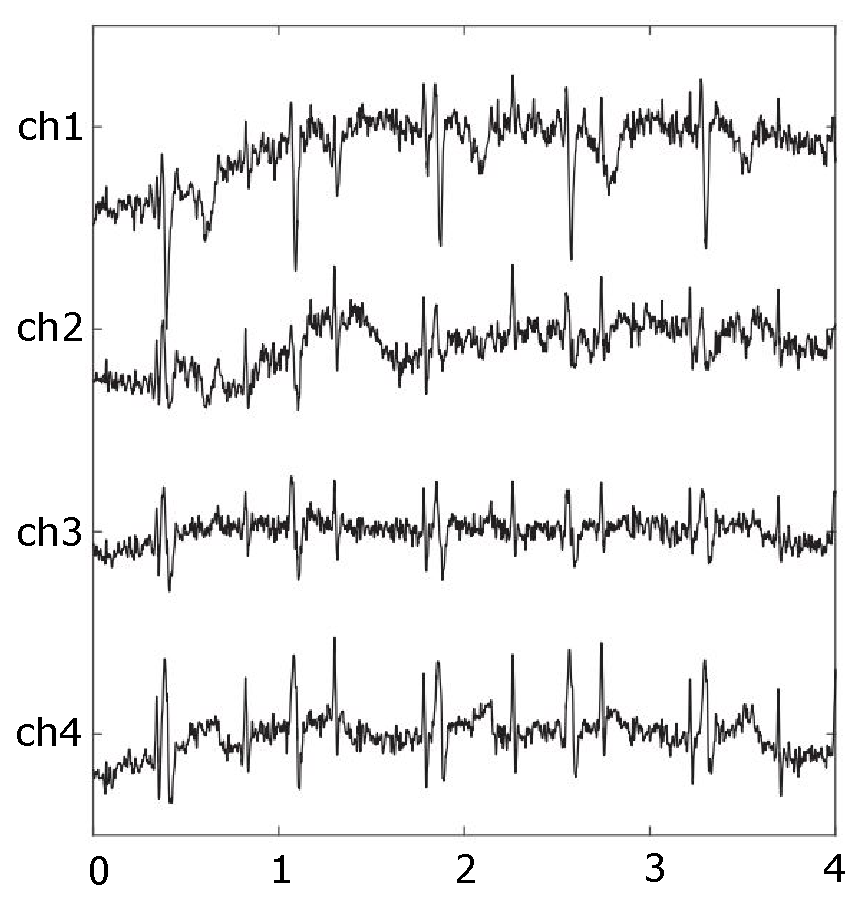
\includegraphics[height=5.20590cm]{./images/mEKG_fEKG.eps}
  \begin{center} (a)
     \end{center}
 \end{minipage} \hfill
   \begin{minipage}[t]{5cm}
    \centering
 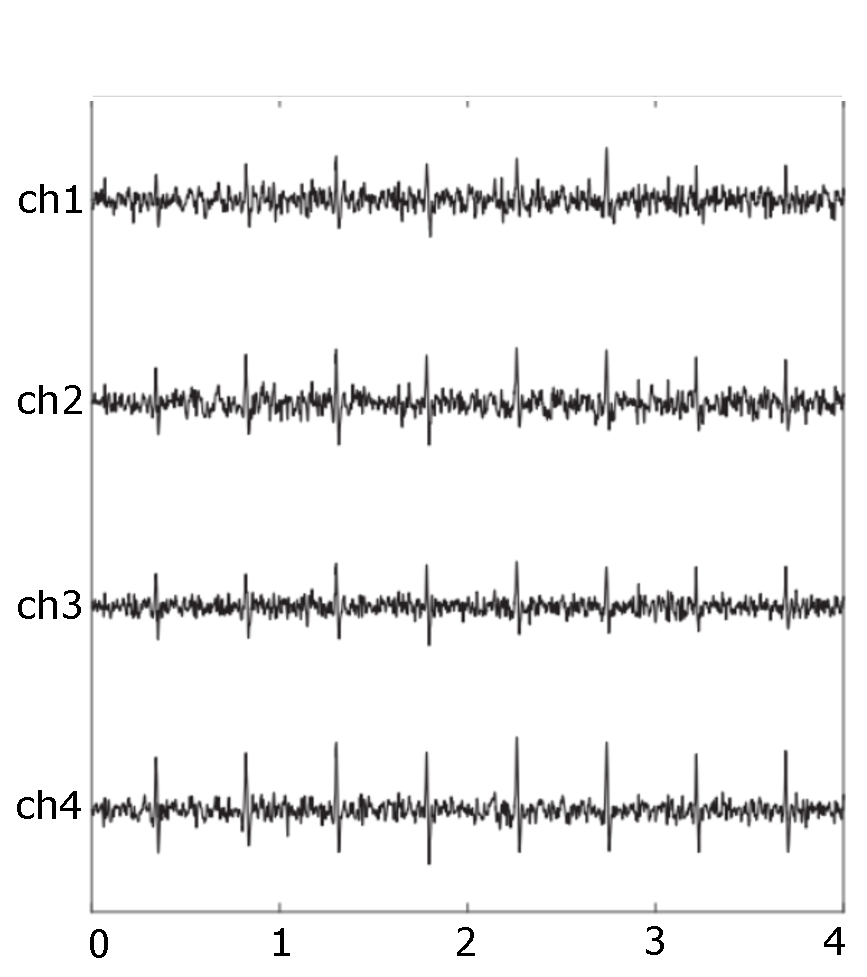
\includegraphics[height=5.64585cm]{./images/fEKG.eps}
  \begin{center} (b)
     \end{center}
 \end{minipage} \hfill
 \caption{{(a) fEKG, überlagert von mEKG, nach \cite{warmerdam2018hierarchical}; (b) fEKG mit ausgefiltertem mEKG, nach \cite{warmerdam2018hierarchical}.\label{fig:fEKG}}}
\end{figure}

%Erklärung EKG
%Paper1:
%nicht-invasiv: Elektroden auf dem Abdomen der Mutter -> schwaches fECG-Signal, das vom starken ECG-Signal der Mutter überlappt wird
%R-Wellen sind gut erkennbar, wird genutzt um andere Methoden zu validieren

%Paper2:
%liefert Information zu fetalem Puls + Information zu fetalem Sauerstoffmangel (ergibt sich aus R-Spitzen)
%invasiv: Platzierung der Elektroden an der fetalen Kopfhaut; kann nur bei der Geburt durchgeführt werden
%nicht-invasiv: schlechte SignalToNoise-Ratio; Rest: s.o.; zwischen 28-32 Wochen umgibt den Fötus eine Membran, die das Signal weiter abschwächt
%Angabe von Papern, die sich mit der Unterdrückung des maternalen ECGs beschäftigen (template substraction, adaptive filtering, blind source separation,...)
%Angabe von Papern, die sich mit der Detektion der R-Spitze beschäftigen; Problem: niedrige SNR, Position des Fötus ist unbekannt und kann variieren
%Angabe von Papern mit Nachbearbeitungsschritten für die R-Spitzen-Detektion
%adaptive Mehrkanal-R-Peak-Detektionsmethode mit Kombination von EKG-Kurven und HR-Informationen

%Paper3:
%Referenz 1 über Algorithmen zur fECG Signal Detektion
%Methode zur R-Spitzen-Detektion im nichtinvasiven ECG

%Paper5:
%Angabe von Papern zu Methoden zur ECG-Extraction (spatial filtering, adaptive filtering, template substraction, independent component analysis)
%langzeitmonitoring ist trotzdem nicht möglich, durch hohe rechnerische Komplexität
%Methode zur R-Spitzen-Detektion im nichtinvasiven ECG

\subsection{Phonokardiographie}
\label{phono}

\paragraph{Beschreibung der Untersuchung}

Beim fetalen Phonokardiogramm (fPKG) werden mithilfe eines Mikrophons und eines Schallverstärkers die fetalen Herztöne aufgezeichnet.
Dies erfolgt entweder über indirekte Kopplung, bei der eine Kuppel auf den Brustkorb aufgesetzt wird, wodurch eine abgeschlossene Luftkammer entsteht.
Über diese werden Schwingungen vom Brustkorb an die Messkuppel weitergegeben.
Dabei können durch unzureichende Abdichtung der Kuppel auf dem Brustkorb Störgeräusche entstehen.
Eine weitere Möglichkeit der Messung erfolgt über einen Stempel, der direkt auf den Brustkorb aufgedrückt wird.

Das dadurch aufgezeichnete Tonsignal kann als grafische Kurve dargestellt werden.
Das Tonsignal beinhaltet zwei wesentliche Komponenten: das Schlussgeräusch der Mitral- und Trikuspidalklappen ($S1$) und das Schlussgeräusch der Aorten- und der Pulmonalklappen ($S2$).
Dabei ist das Segment zwischen dem $S1$ und dem $S2$ Signal das systolische Zeitintervall und das Segment zwischen dem S2 und S1 Signal das diastolische \cite{kovacs2011fetal}.
Dies ist für zwei Zyklen in Abbildung \ref{fig:fPCG} dargestellt.

\begin{figure}[b]
 \centering
 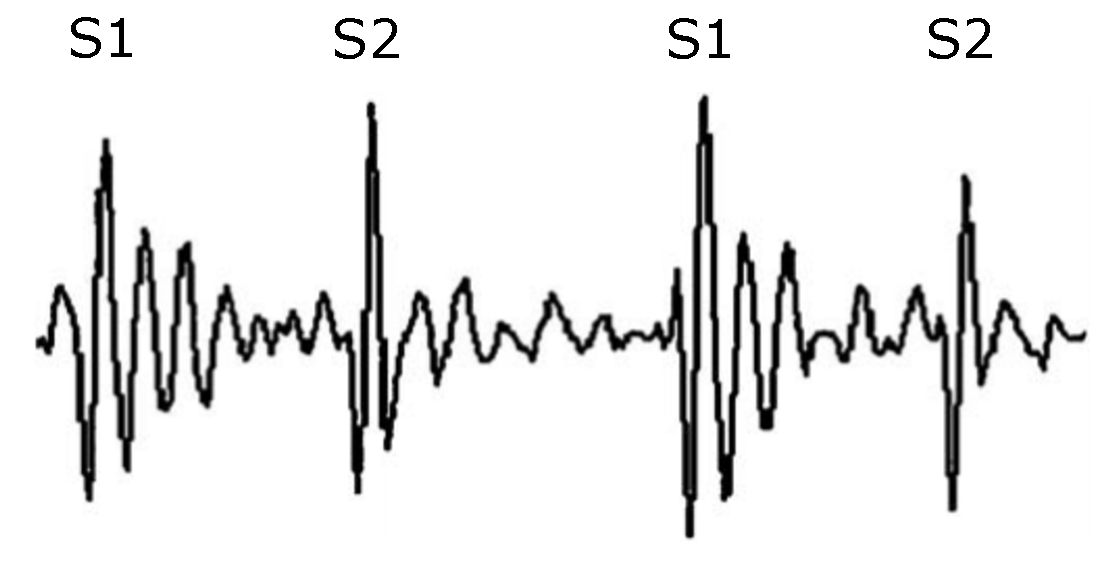
\includegraphics[height=3.19505cm]{./images/fPCG.eps}
\hfill
 \caption{{Normales fPCG Signal mit Markierung der S1 und S2 Signaltöne, nach \cite{kovacs2011fetal}.\label{fig:fPCG}}}
\end{figure}

Dabei ist zu beachten, dass das Signal je nach Scheitelpunktposition des Fötus vom Fruchtwasser gedämpft werden kann, da der Schall bei der $Vertex$ $Occupant$ $Posterior$ (VOP) Position des Fötus, bei der die Vorderseite des Fötus der Messkuppel zugewandt ist, einen weiteren Weg zurücklegen muss, als bei der $Vertex$ $Occupant$ $Anterior$ (VOA) Position, bei der die Rückseite des Fötus der Messkuppel zugewandt ist.
Problematisch kann dabei auch eine mögliche Fettleibigkeit der Mutter sein \cite{adithya2017trends}.
Zudem unterscheidet sich das fPCG signifikant von dem eines Erwachsenen, da das fetale Herz über eine weitere Öffnung zwischen den beiden Herzvorhöfen verfügt, das $foramen$ $ovale$, das einen Blutstrom vom Lungenkreislauf in den Körperkreislauf ermöglicht.
Das Signal ist außerdem von den maternalen Geweben gedämpft, sodass es eine niedrige Amplitude und eine schmale Frequenz besitzt.
Die Frequenz des Signals variiert je nach Gewicht des Fötus und je nach Schwangerschaftswoche.
Des Weiteren wird das Signal von den maternalen Herzgeräuschen überlagert, welche allerdings durch einen Tiefpassfilter ausgesondert werden können, da ihre Frequenz größtenteils unter 25Hz liegt.
Weitere Beeinträchtigungen des Signals entstehen durch die Bewegungen des Fötus, wie zum Beispiel die Atembewegungen, Bewegungen der Extremitäten oder durch Schluckauf, oder durch die maternale Atmung, Muskelbewegung oder Geräusche von umliegenden Organen.
Diese Störungen können allerdings bei korrekter Positionierung der Messkuppel vernachlässigt werden \cite{kovacs2011fetal}.

\paragraph{Messbare Parameter}

Das fPKG zeichnet direkt die fetalen Herztöne (fHS) auf.
Daraus lassen sich T\textsubscript{bb} und fHR berechnen, indem man von jedem Herzschlag einen Referenzpunkt ermittelt.
Dieser ist normalerweise der $S1$ Ton, da dieser für gewöhnlich die höchste Amplitude besitzt und so leicht detektierbar ist.
Zudem können durch das fPKG Herzsgeräusche ermittelt werden, welche auf einen angeborenen Herzfehler schließen lassen.
Über die fHS kann außerdem die sogenannte $Split$ $Time$ (ST) festgestellt werden, die entsteht, wenn sich beispielsweise die Mitral- und die Trikuspidalklappe, die sich normalerweise synchron schließen, zeitversetzt schließen, sodass sich das $S1$ Signal in zwei Töne spaltet.
Des Weiteren kann durch die Spektralanalyse der fHR-Variabilität intrauterine Wachstumsretardierung gezeigt werden.
Im Umkehrschluss bedeutet das, dass durch Langzeitmonitoring des fHR das intrauterine Wachstum überwacht werden kann.
Ebenso kann durch die Variabliltät der fHR das Wachstum des fetalen Nervensystems verfolgt werden.
Da das fPKG über längere Zeitintervalle durchgeführt werden kann, können die fetalen Atembewegungen aufgezeichnet werden.
Diese treten nur kurzzeitig und überlagert von anderen fetalen Bewegungen überlagert auf und sind daher schwer zu identifizieren  \cite{kovacs2011fetal}.

\paragraph{Verarbeitung der Messwerte}

Um die fHR zu ermitteln, müssen primär die Referenzpunkte der Herzschläge detektiert werden.
Dies erfolgt generell über zwei Methoden: durch die Autokorrelation der Intensitätskurve oder durch die Wavelet Transform.
Teilweise werden auch beide Methoden in Kombination verwendet, da das $S1$ Geräusch in den meisten Fällen eine niedrige Intensität besitzt.
Bei der Autokorrelation werden die periodischen Eigenschaften des Herzsignals ausgenutzt, indem ein Abschnitt der Intensitätskurve mit dem folgenden Abschnitt unter Verwendung eines sich bewegenden Fensters verglichen wird.
Die Schlagzeit ergibt sich aus dem Zeitunterschied der ähnlichsten Punkte.
Bei der Wavelet Transform wird generell die Daubechies-Funktion \cite{daubechies1988orthonormal} verwendet, die an Maßstab und Verschiebung des Signals angepasst wird.
Dabei ist zu beachten, dass diese Methode falsche kardiale Signale detektiert, wenn Störungen ähnliche Frequenzeigenschaften besitzen wie das eigentlich gesuchte $S1$ Signal.
Nach der Detektion der Referenzpunkte erfolgt ein Herausfiltern der maternalen Geräusche und anderer Störsignale \cite{kovacs2011fetal}.
Zur Berechnung der fHR gibt es mehrere Ansätze \cite{godinez2003line, kovacs2000rule, talbert1986wide, jimenez2001performance, tan2000real, kovacs1998improved}, wobei viele nicht mit verrauschten Aufnahmen umgehen konnten.

%\cite{kovacs2011extended}

%Erklärung PCG
%akustisches Signal des Fötus wird gestört durch fetale Bewegungen, Herz der Mutter, Verdauungssystem
%öglichkeiten zur Rauschunterdrückung:
%Paper1: wavelet transform
%paper1: matching pursuit
%Paper1: model-based individual correlation

\subsection{Ultraschall Kardiotokographie}
\label{ctg}

\paragraph{Beschreibung der Untersuchung}

Ultraschall ist aktuell für die meisten messbaren Parameter ab der 28. Schwangerschaftswoche, wie fetale Atmung, fetaler Schluckauf, fHR oder den Blutfluss in der Nabelschnur, der Goldstandard.
Verwendet man diesen in Kombination mit einem Tokodynamometer, spricht man von der Ultraschall Kardiotokographie (CTG).
Dies erfolgt größenteils während der Geburt, um die fHR und die Wehentätigkeit (mUC) zu überwachen, wobei mit einem Differenzdruckmesser die Änderung der Bauchspannung während einer Wehe gemessen wird.
Das CTG ist zum Langzeitmonitoring nicht geeignet, da der Ultraschallkopf häufig neu ausgerichtet werden muss und zudem durchgängig ein speziell ausgebildeter Bediener zur Datenauswertung anwesend sein muss.
Zudem ist Ultraschall hochempfindlich gegenüber Bewegungen, sowohl maternalen als auch fetalen, da diese die Reflexion des Schalls beeinträchtigen.
Des Weiteren wird der Fötus bei dieser Untersuchung Strahlung ausgesetzt und der aktuellen Literatur ist nicht zu entnehmen, inwieweit dies sicher für den Fötus ist \cite{adithya2017trends}.

\paragraph{Messbare Parameter}

Über das CTG wird simultan die fHR und die Wehentätigkeit gemessen.
Über die Kurzzeitvariablilität (STV) der fHR lässt sich Aufschluss auf den Blutfluss der Nabelschnur gewinnen und damit auf die Sauerstoffversorgung des Fötus.
Weiterhin kann die Grundlinie der fHR bestimmt werden.
Der Abfall der fHR gefolgt von einer Gebärmutterkontraktion lässt auf eine abnormale Situation der Schwangerschaft schließen.
Über die Analyse der fHR können des Weiteren intrauterine Wachstumsstörungen oder das Wachstum des fetalen Nervensystems überwacht werden \cite{kovacs2011fetal}.

\paragraph{Verarbeitung der Messwerte}

Das CTG zeichnet sich durch eine niedrige Spezifität aus, da die Reflexion des Ultraschalls durch Bewegungen wie die Herzkammerkontraktionen oder Atembewegungen verändert wird, was zu ungenauen fHR-Messungen führt.
Daraus folgt, dass für die weitere Verarbeitung der Messwerte mit unpräzisen Schlagzeiten gearbeitet werden muss, sodass die weitere Analyse zu einer hohen Fehlerfortpflanzung führen würde \cite{kovacs2011fetal}.

%Das Ultraschall Kardiotokogramm (CTG) ist seit 1960 das am häufigsten durchgeführte Verfahren zur fetalen Überwachung \cite{warmerdam2018hierarchical}.

%Das Verfahren liefert sowohl Information über die fetale Herzrate (fHR) als auch über die uterine Aktivität \cite{warmerdam2018hierarchical}.

%Allerdings verfügt das Verfahren über eine geringe Spezifität, was zu einer unnötig hohen Anzahl an operativen Geburten führt \cite{warmerdam2018hierarchical}.



%Erklärung CTG
%Paper1:
%ultrasound doppler technique: ungenauigkeiten durch Reflexion an Herzventilen; standard Fehler von 0.42ms und standardabweichung von 4.18ms im Vergleich zu ECG.
%kann nicht verwendet werden, um die STV zu ermitteln
%STV wird zur Ermittlung anderer Daten benötigt, also eher schlecht verwendbar

%Paper2:
%niedrige Spezifität

\section{Vergleich der fetalen Untersuchungsmethoden}
\label{signal}

Tabelle \ref{tab:methods} liefert einen kurzen Überblick über die Parameter, die mit den verschiedenen Untersuchungsmethoden beobachtet werden können.

\begin{table}[h]
 \setlength{\extrarowheight}{0.2cm}
\centering
\resizebox{\columnwidth}{!}{%
\begin{tabular}{|c|ccc|} 
\hline
Untersuchung & fEKG & fPKG & CTG \\ 
\hline
\begin{tabular}[c]{@{}c@{}}messbare\\ Parameter \end{tabular} & fHR & fHS & fHR, mUC \\
\begin{tabular}[c]{@{}c@{}}ableitbare\\ Parameter \end{tabular} & \begin{tabular}[c]{@{}c@{}}T\textsubscript{bb}, STV, \\ fetale \\Sauerstoffdefizite,\\ intrauterine \\Wachstumsstörungen, \\ Wachstum des \\fetalen Nervensystems \end{tabular} & \begin{tabular}[c]{@{}c@{}}T\textsubscript{bb}, fHR, STV, \\Herzgeräusche, \\intrauterine \\ Wachstumsstörungen, \\Wachstum des \\ fetalen Nervensystems, \\fetale Atembewegungen \end{tabular} & \begin{tabular}[c]{@{}c@{}}T\textsubscript{bb}, STV, Blutfluss \\über die Nabelschnur,\\ Sauerstoffversorgung\\des Fötus, Mittellinie,\\ intrauterine \\Wachstumsstörungen, \\Wachstum\\ des fetalen Nervensystems \end{tabular} \\
\begin{tabular}[c]{@{}c@{}}Langzeitmonitoring\\ möglich? \end{tabular} & Ja & Ja & Nein \\
\hline
\end{tabular}
}
\caption{Gegenüberstellung der Untersuchungsmethoden.}
\label{tab:methods}
\end{table}

...

%Kriterien: Kosten, technischer Aufwand, messbare Parameter, ableitbare Parameter, langzeitmonitoring möglich

\section{Zusammenfassung}
\label{resume}

...

\section{Ergebnisse und Ausblick}
\label{end}

...

%
%%%%%%%%%%%%%%%%%%%%%%%%%%%%%%%%%%%%%%%%%%%%%%%%%%%%%%%%%%%%%%%%%%%%%%%%%%%%%%%%%%%%
% Literaturverzeichnis
\printbibliography


% Anhang
\appendix
\section{Anhang}
\label{anhang}



\end{document}
